\documentclass{jknotes}
\usepackage{joshkirklin}

\begin{document}

\institution{Cambridge Part III Maths}
\title{Advanced Quantum Field Theory}
\lecturer{David Skinner}
\notetaker{Josh Kirklin}
\date{Lent 2016}

\maketitle
\suggestionsspiel
\tableofcontents

\section{Introduction}
\lecture{15/01/16}
We must do three things to construct a QFT:
\begin{enumerate}
    \item Pick a smooth manifold \(\mathcal{M}\) (which we call \emph{space}, or \emph{spacetime} if it is Lorentzian) in which our QFT is going to live, and choose a metric \(g\) for \(\mathcal{M}\).
        For example:
        \begin{itemize}
            \item In particle physics, \(\mathcal{M}=\RR^4\) and \(g=\) the Minkowski metric \(\eta\).
            \item In statistical physics, \(\mathcal{M}=\RR^4\) and \(g=\) the Euclidean metric \(\delta\).
            \item In string theory, \(\mathcal{M}=\Sigma\), some Riemann surface.
        \end{itemize}
    \item Pick some \emph{fields}. These might be:
        \begin{itemize}
            \item Scalar fields \(\phi^a:\mathcal{M}\rightarrow\RR\), \(a=1,\dots,m\). This is known as a \emph{linear sigma model}.
            \item \(\phi:\mathcal{M}\rightarrow\mathcal{N}\) where \((\mathcal{N},G)\) is a general Riemannian manifold. If \(\mathcal{N}\ne \RR^m\), this is called a \emph{non-linear sigma model}.
                \begin{figure}[H]
                    \centering
                    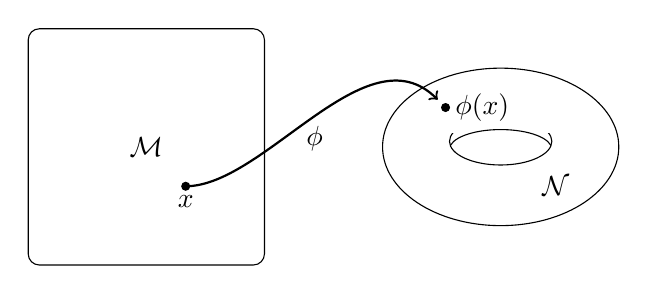
\begin{tikzpicture}
                        \draw[rounded corners](0,0) rectangle (3,3);
                        \node at (1.5,1.5) {\(\mathcal{M}\)};
                        \draw[fill](2,1) circle (0.05) node[below] {\(x\)};

                        \draw(6,1.5) ellipse (1.5 and 1);
                        \begin{scope}
                            \clip(6,1.57) ellipse (0.65 and 0.3);
                            \draw(6,1.47) ellipse (0.65 and 0.25);
                        \end{scope}
                        \begin{scope}
                            \clip(4.5,0) rectangle (7.5,1.67);
                            \draw(6,1.57) ellipse (0.65 and 0.3);
                        \end{scope}
                        \draw[fill](5.3,2) circle (0.05) node[right] {\(\phi(x)\)};
                        \node at (6.7,1) {\(\mathcal{N}\)};

                        \draw[thick,->](2,1) .. controls (3,1) and (4.3,3) .. (5.2,2.1) node[midway, below] {\(\phi\)};
                    \end{tikzpicture}
                \end{figure}
            \item \(\psi\) a (Dirac) spinor on \(\mathcal{M}\).
            \item Gauge fields \(A_\mu(x)\) (taking values in \(\Omega^1(\mathcal{M},\mathcal{L}(G))\), i.e. the set of all 1-forms on \(\mathcal{M}\) with coefficients in the Lie algebra of some Lie group \(G\)).
        \end{itemize}
    \item We must pick an action \(S:\mathcal{C}\rightarrow\RR\), where \(\mathcal{C}\) is the space of fields. For example:
        \begin{itemize}
            \item For a scalar field \(\phi\):
                \begin{equation}
                    S[\phi] = \int_\mathcal{M}\dd[d]{x}\sqrt{g}\Big[ \underbrace{\frac{g^{\mu\nu}}{2}\partial_\mu\phi\partial_\nu\phi}_{\text{kinetic term}}-\underbrace{V(\phi)}_{\mathclap{\substack{\text{potential}\\\text{term}}}} \Big]
                \end{equation}
            \item For a gauge field \(A\):
                \begin{equation}
                    S[A] = \frac{1}{4e^2}\int\dd[d]{x}\sqrt{g}g^{\mu\nu}g^{\rho\sigma}\underbrace{(F_{\mu\rho},F_{\nu\sigma})}_{\text{Killing form}}
                \end{equation}
        \end{itemize}
        In general, the action, even for a scalar, can be the integral of an arbitrary differential polynomial in the fields:
        \begin{equation}
            S[\phi] = \int \underbrace{\mathcal{L}(\phi,\partial^p\phi)}_{\mathclap{\substack{\text{polynomial in }\phi\\\text{and all derivatives}}}} \sqrt{g} \dd[d]{x}
        \end{equation}
\end{enumerate}

\section{QFT in zero dimensions}
If \(\dim \mathcal{M} = 0\) and \(\mathcal{M}\) is connected, then \(\mathcal{M}=\{\text{pt}\}\). We'll choose our fields to be \(\phi:\{\text{pt}\}\rightarrow\RR\) (i.e. \(\phi\in\RR\)).

The basic object we want to compute (in any QFT) is the partition function:
\begin{equation}
    Z = \int_\mathcal{C} \Dd{\phi} e^{-S[\phi]}
\end{equation}
which in this case is just:
\begin{equation}
    Z = \int_\RR \dd{\phi} e^{-S(\phi)}
\end{equation}
We'll assume that \(e^{-S(\phi)}\) decays sufficiently rapidly as \(|\phi|\rightarrow\infty\) that this integral converges. In practice, we take \(S(\phi)\) to be an even degree polynomial in \(\phi\), for example:
\begin{equation}
    S(\phi) = \frac{m^2}{2}\phi^2 + \frac{\lambda}{4!}\phi^4
\end{equation}
In this case \(Z=Z(m,\lambda,\dots)\) is a function of all the coupling constants in \(S(\phi)\). For example:
\begin{equation}
    Z(m^2) = \int_\RR \dd{\phi}e^{-m^2\phi^2/2} = \frac{\sqrt{2\pi}}{m}
\end{equation}
If we include more terms, integrals become hard to solve:
\begin{equation}
    Z(m^2,\phi) = \int_\RR e^{-m^2\phi^2/2-\lambda\phi^4/4!}
\end{equation}
We can try to evaluate this perturbatively in \(\lambda\):
\begin{align}
    Z(m^2,\phi) &= \int \dd{\phi} \left( e^{-m^2\phi^2/2} \sum_{n=0}^\infty \left( \frac{-\lambda}{4!} \right)^n\frac{\phi^{4n}}{n!} \right)\\
    &\stackrel{?}{\sim} \sum_{n=0}^\infty \left( \frac{-\lambda}{4!} \right)^n\frac{1}{n!}\int\dd{\phi}\phi^{4n}e^{-m^2\phi^2/2}
\end{align}
This integral can't possibly converge as a power series in \(\lambda\). In fact this is an asymptotic series\footnote{
    Recall: \(\sum_{n=0}^\infty a_n\lambda^n\) is an asymptotic series for \(Z(\lambda)\) if:
    \begin{equation}
        \lim_{\lambda\rightarrow 0} \frac{|Z(\lambda)-\sum_{n=0}^Na_n\lambda^n|}{\lambda^N}=0 \quad \text{for all } N\in\NN
    \end{equation}
} for \(Z(m^2,\lambda)\). Feynman diagram expansions in QFT are (almost) always asymptotic expansions. It can be shown :
\begin{align}
    Z(m^2\lambda) &\sim \frac{\sqrt{2\pi}}{m}\left[ 1-\frac{\lambda}{8m^4} + \frac{35}{384}\frac{\lambda^2}{m^4} + \dots \right]
\end{align}
Inductively, the coefficient of \(\lambda^n\) is \(\frac{1}{(4!)^nn!}\times\frac{(4n)!}{4^n(2n)!}\). We expect \(\frac{1}{(4!)^nn!}\) as the coefficient in a series expansion. \(\frac{(4n)!}{4^n(2n)!}\) is the number of ways of joining \(4n\) objects into pairs.

\subsection{Feynman rules}
\lecture{18/01/16}
We represent each term in the asymptotic series as a graph. Each propagator %
\raisebox{.2\baselineskip}{\begin{tikzpicture}
    \draw (0,0) -- (1,0);
\end{tikzpicture}} %
contributes a factor of \(\frac{1}{m^2}\), and each vertex %
\raisebox{-.5\height+.2\baselineskip}{
\begin{tikzpicture}[scale=0.3]
    \draw (0,0) -- (1,1);
    \draw (1,0) -- (0,1);
    \fill (0.5,0.5) circle (0.15);
\end{tikzpicture}} %
contributes a factor of \(-\lambda\). For the partition function, we just want vacuum graphs, so we have no external legs. Feynman rules tell us to draw all such graphs, imagining that the lines emanating from each vertex are labelled. For example, at first order (one vertex), we can make the following graphs:
\begin{figure}[H]
    \centering
    \begin{tikzpicture}
        \draw[thick,->] (-3.2,0) -- (-2.3,0);
        \begin{scope}[shift={(-4.5,0)}]
            \draw (-0.5,-0.5) -- (0.5,0.5);
            \draw (-0.5,0.5) -- (0.5,-0.5);
            \fill (0,0) circle (0.05);
            \node[above] at (0.5,0.5) {1};
            \node[below] at (0.5,-0.5) {2};
            \node[below] at (-0.5,-0.5) {3};
            \node[above] at (-0.5,0.5) {4};
        \end{scope}
        \begin{scope}[shift={(7,0)}]
            \draw (0,0) arc (135:-225:1);
            \fill[white] ({sqrt(2)},0) circle (0.1);
            \draw (0,0) arc (225:-135:1);
            \fill (0,0) circle (0.05);
            \node[above] at (0.5,0.3) {1};
            \node[below] at (0.5,-0.3) {2};
            \node[left] at (-0.3,-0.5) {3};
            \node[left] at (-0.3,0.5) {4};
        \end{scope}
        \begin{scope}[shift={(3.5,0)},rotate=-90]
            \draw (0,0) .. controls (2,2) and (2,-2) .. (0,0)
                        .. controls (-2,2) and (-2,-2) .. cycle;
            \fill (0,0) circle (0.05);
            \node[right] at (-0.5,0.5) {1};
            \node[right] at (0.5,0.5) {2};
            \node[left] at (0.5,-0.5) {3};
            \node[left] at (-0.5,-0.5) {4};
        \end{scope}
        \begin{scope}
            \draw (0,0) .. controls (2,2) and (2,-2) .. (0,0)
                        .. controls (-2,2) and (-2,-2) .. cycle;
            \fill (0,0) circle (0.05);
            \node[above] at (0.5,0.5) {1};
            \node[below] at (0.5,-0.5) {2};
            \node[below] at (-0.5,-0.5) {3};
            \node[above] at (-0.5,0.5) {4};
        \end{scope}
    \end{tikzpicture}
\end{figure}
Hence, the first order term in the expansion is given by:
\begin{figure}[H]
    \centering
    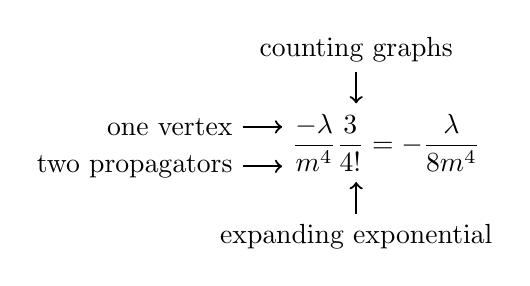
\begin{tikzpicture}
        \node[right] at (0,0) {\(\displaystyle\frac{-\lambda}{m^4}\frac{3}{4!} = - \frac{\lambda}{8m^4}\)};

        \draw[thick,<-] (0,0.2) -- (-0.5,0.2) node[left] {one vertex};
        \draw[thick,<-] (0,-0.3) -- (-0.5,-0.3) node[left] {two propagators};
        \draw[thick,<-] (0.94,0.5) -- (0.94,0.9) node[above] {counting graphs};
        \draw[thick,<-] (0.94,-0.5) -- (0.94,-0.9) node[below] {expanding exponential};
    \end{tikzpicture}
\end{figure}
Drawing \emph{all} of these graphs can be very laborious. There is a shortcut.

Let \(D_n\) be the set of all labelled graphs with \(n\) vertices. Each will come with a factor of \(-\lambda^n\), but as topological (i.e. unlabelled) graphs, we've overcounted, and we should account for this. \(D_n\) is naturally acted on by the group \((S_4)^n\times S_n\), where the \(S_4\)s act by permuting the labels at each vertex, and the \(S_n\) acts be permuting the vertices themselves. This group has order \((4!)^nn!\) and so the weight of Feynman graphs with
\(n\) vertices is \(|D_n|/(4!)^nn!\).

It's useful to rewrite this in the following way. Let \(\Gamma\) be an orbit of \(G_n=(S_4)^n\times S_n\) in \(D_n\), i.e. \(\Gamma\) is a topologically distinct unlabelled graph. As an example, the following two graphs are distinct:
\begin{figure}[H]
    \centering
    \begin{tikzpicture}
        \begin{scope}
            \draw (0,0) .. controls (1,0.9) and (2,0.9) .. (3,0);
            \draw (0,0) .. controls (1,0.3) and (2,0.3) .. (3,0);
            \draw (0,0) .. controls (1,-0.3) and (2,-0.3) .. (3,0);
            \draw (0,0) .. controls (1,-0.9) and (2,-0.9) .. (3,0);
            \fill (0,0) circle (0.05);
            \fill (3,0) circle (0.05);
        \end{scope}
        \node at (4.3,0) {\(\not\sim\)};
        \begin{scope}[shift={(6,0)}]
            \fill (1,0) circle (0.05);
            \fill (4,0) circle (0.05);
            \draw (1,0) .. controls (2,1) and (3,1) .. (4,0) 
                        .. controls (6,-2) and (6,2) .. (4,0)
                        .. controls (3,-1) and (2,-1) .. (1,0)
                        .. controls (-1,2) and (-1,-2) .. cycle;
        \end{scope}
    \end{tikzpicture}
\end{figure}
Also, let \(\mathcal{O}_n\) be the set of these orbits (i.e. the set of topologically distinct graphs with \(n\) vertices). Then the orbit-stabilizer theorem states that:
\begin{equation}
    \frac{|D_n|}{|G_n|} = \sum_{\Gamma\in\mathcal{O}_n}\frac{1}{|\text{Aut}\,\Gamma|}
\end{equation}
where \(\text{Aut}\,\Gamma\) is the set of elements in \(G_n\) that fix \(\Gamma\). \(|\text{Aut}\,\Gamma|\) is sometimes called the \emph{symmetry factor}.

Thus the weight of the \(n\) vertex contribution to the asymptotic series for \(Z(m,\lambda)\) is:
\begin{equation}
    \frac{(-\lambda)^n}{m^{4n}}\sum_{\Gamma\in\mathcal{O}_n}\frac{1}{|\text{Aut}\,\Gamma|}
\end{equation}
and therefore we have:
\begin{align}
    \frac{Z(m,\lambda)}{Z(m,0)} &= \sum_{n=0}^\infty \left( \frac{(-\lambda)^n}{m^{4n}}\sum_{\Gamma\in\mathcal{O}_n}\frac{1}{|\text{Aut}\,\Gamma|} \right) \\
    &= \sum_\Gamma \frac{1}{|\text{Aut}\,\Gamma|} \frac{(-\lambda)^{|v(\Gamma)|}}{(m^2)^{|e(\Gamma)|}}
\end{align}
where \(|e(\Gamma)|\) is the number of edges, and \(|v(\Gamma)|\) is the number of vertices.

As a sanity check, lets use this to calculate the first few terms:
\begin{figure}[H]
    \centering
    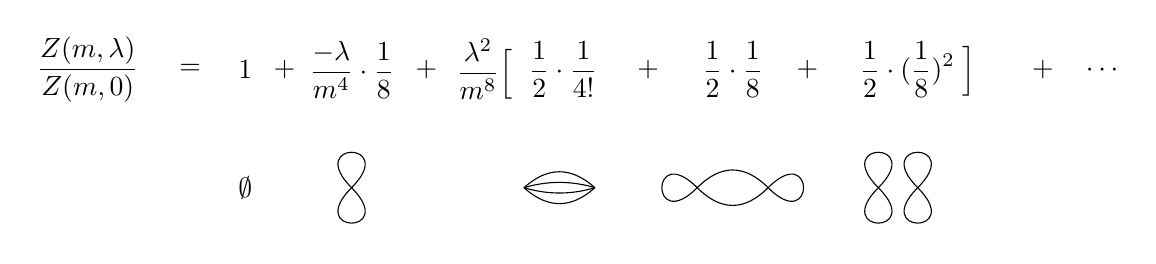
\begin{tikzpicture}
        \node at (0,0) {\(\displaystyle \frac{Z(m,\lambda)}{Z(m,0)}\)};
        \node at (1.3,0) {\(=\)};

        \begin{scope}[shift={(2,0)}]
            \node at (0,0) {1};
            \node at (0,-1.5) {\(\emptyset\)};
        \end{scope}
        \node at (2.5,0) {\(+\)};
        \begin{scope}[shift={(3.35,-1.5)}]
            \draw[rotate=90, scale=0.3] (0,0) .. controls (2,2) and (2,-2) .. (0,0)
                        .. controls (-2,2) and (-2,-2) .. cycle;
            \node at (0,1.5) {\(\displaystyle \frac{-\lambda}{m^4}\cdot\frac{1}{8}\)};
        \end{scope}
        \node at (4.3,0) {\(+\)};
        \begin{scope}[shift={(5.04,0)}]
            \begin{scope}[shift={(0.5,-1.5)},scale=0.3]
                \draw (0,0) .. controls (1,0.9) and (2,0.9) .. (3,0);
                \draw (0,0) .. controls (1,0.3) and (2,0.3) .. (3,0);
                \draw (0,0) .. controls (1,-0.3) and (2,-0.3) .. (3,0);
                \draw (0,0) .. controls (1,-0.9) and (2,-0.9) .. (3,0);
            \end{scope}
            \begin{scope}[shift={(2.4,-1.5)}]
                \draw[scale=0.3] (1,0) .. controls (2,1) and (3,1) .. (4,0) 
                            .. controls (6,-2) and (6,2) .. (4,0)
                            .. controls (3,-1) and (2,-1) .. (1,0)
                            .. controls (-1,2) and (-1,-2) .. cycle;
            \end{scope}
            \begin{scope}[shift={(5,-1.5)}]
                \draw[rotate=90, scale=0.3] (0,0) .. controls (2,2) and (2,-2) .. (0,0)
                            .. controls (-2,2) and (-2,-2) .. cycle;
            \end{scope}
            \begin{scope}[shift={(5.5,-1.5)}]
                \draw[rotate=90, scale=0.3] (0,0) .. controls (2,2) and (2,-2) .. (0,0)
                            .. controls (-2,2) and (-2,-2) .. cycle;
            \end{scope}
            \node at (0,0) {\(\displaystyle\frac{\lambda^2}{m^8}\Big[\)};
            \node at (1,0) {\(\displaystyle\frac{1}{2}\cdot\frac{1}{4!}\)};
            \node at (2.075,0) {\(+\)};
            \node at (3.15,0) {\(\displaystyle\frac{1}{2}\cdot\frac{1}{8}\)};
            \node at (4.1,0) {\(+\)};
            \node at (5.5,0) {\(\displaystyle\frac{1}{2}\cdot\qty(\frac{1}{8})^2\;\Big]\)};
            \node at (7.5,0) {\(+\quad\cdots\)};
        \end{scope}
    \end{tikzpicture}
\end{figure}
which if we do the arithmetic will lead to agreement with the above.

More generally we may have several types of field \(\phi_i\), each with some propagator \(\frac{1}{P_i}\). These may interact through many types of vertices \(\alpha\), each with coupling constant \(\lambda_\alpha\). Then the partition function has an asymptotic series expansion:
\begin{align}
    \frac{Z}{Z|_{\lambda_\alpha=0}} &= 
    \sum_\Gamma \frac{1}{|\text{Aut}\,\Gamma|}\frac{\prod_\alpha(-\lambda_\alpha)^{|v_\alpha(\Gamma)|}}{\prod_i P_i^{|e_i(\Gamma)|}} \\
    &= \exp \qty( \sum_{\Gamma\text{ connected}} \frac{1}{|\text{Aut}\,\Gamma|}\frac{\prod_\alpha(-\lambda_\alpha)^{|v_\alpha(\Gamma)|}}{\prod_i P_i^{|e_i(\Gamma)|}} ) \\
    &= \exp(W)
\end{align}
where we use the last line to define \(W\), the (Helmholtz) free energy.

\subsection{Schwinger-Dyson equations}
Trivially, \(Z = \int_\RR\dd{\phi}e^{-S(\phi)} = \int_\RR\dd{(\phi+\epsilon)}e^{-S(\phi+\epsilon)}\) for any constant \(\epsilon\). By translational invariance of the measure, \(\dd{(\phi+\epsilon)} = \dd{\phi}\), so we have:
\begin{equation}
    Z = \int_\RR\dd{\phi}e^{-S(\phi+\epsilon)} = \int_\RR\dd{\phi}e^{-S(\phi)}\left[ 1 - \epsilon\pdv{S}{\phi} \right] + O(\epsilon^2)
\end{equation}
If we compare this to our original expression for \(Z\), we see \(Z = Z - \epsilon\int\dd{\phi}e^{-S}\pdv{S}{\phi}+O(\epsilon^2)\), which implies:
\begin{equation}
    \expval{\pdv{S}{\phi}} = 0
\end{equation}
where we take the normal definition of the expectation of a function \(f(\phi)\) for a given partition function:
\begin{equation}
    \expval{f(\phi)} = \frac{1}{Z}\int\dd{\phi}e^{-S(\phi)}f(\phi)
\end{equation}
This is essentially Ehrenfest's theorem: the expectation value of the classical equation of motion holds. For example, if \(S=\frac{m^2\phi^2}{2} + \frac{\lambda\phi^4}{4!}\), then we have \(\expval{\pdv{S}{\phi}} = \expval{m^2\phi+\frac{\lambda\phi^3}{3!}} = 0\).

\lecture{20/01/16}
However, to probe how the fluctuations take us away from the classical equations of motion, we should compute more general correlation functions. We let \(f:\mathcal{C}\rightarrow\RR\) and compute \(\expval{f}\):
\begin{align}
    \expval{f} &= \frac{1}{Z}\int_\RR\dd{\phi}e^{-S(\phi)}f(\phi) \\
    &= \frac{1}{Z} \int_\RR\dd{(\phi+\epsilon)} e^{-S(\phi+\epsilon)}f(\phi+\epsilon) \\
    &= \frac{1}{Z} \int_\RR \dd{\phi} e^{-S(\phi)} \left( f-\epsilon\pdv{S}{\phi}f + \epsilon\pdv{f}{\phi} \right) + O(\epsilon^2)
\end{align}
The \(0^\text{th}\) order term is just \(\expval{f}\), so comparing to the left hand side we have:
\begin{equation}
    \expval{\pdv{S}{\phi}f(\phi)} = \expval{\pdv{f}{\phi}}
\end{equation}
So the classical equation of motion \(\pdv{S}{\phi}=0\) does not hold in the presence of so-called \emph{operator insertions}.

\subsection{Effective Theories}
Let's consider a \(d=0\) QFT involving two fields \((\phi,\chi)\in\RR^2\) with the following action (chosen for its simplicity):
\begin{equation}
    S(\phi,\chi) = \frac{m^2}{2}\phi^2 + \frac{M^2}{2}\chi^2 + \frac{\lambda}{4}\phi^2\chi^2
\end{equation}
With this action we have a different set of Feynman rules, contributing the following factors to each diagram:
\begin{figure}[H]
    \centering
    \begin{tikzpicture}
        \draw (0,0) node[left] {\(\phi\)} -- (2,0) node[right] {\(\phi\)};
        \node[below] at (1,0) {\(\frac{1}{m^2}\)};
        \draw[dashed] (4,0) node[left] {\(\chi\)} -- (6,0) node[right] {\(\chi\)};
        \node[below] at (5,0) {\(\frac{1}{M^2}\)};
        \draw (9,0) arc (-90:-45:1.5) node[above] {\(\phi\)};
        \draw (9,0) arc (-90:-135:1.5) node[above] {\(\phi\)};
        \draw[dashed] (9,0) arc (90:135:1.5) node[below] {\(\chi\)};
        \draw[dashed] (9,0) arc (90:45:1.5) node[below] {\(\chi\)};
        \draw[fill] (9,0) circle (0.03) node[below] {\(-\lambda\)};
    \end{tikzpicture}
\end{figure}
We can use these to compute the partition function. Let \(Z_0 = Z|_{\lambda=0}\). We have:
\begin{align}
    \log\frac{Z}{Z_0} &= \sum \text{connected vacuum diagrams} \\
    &
    \begin{matrix}
        \;= & 
        \raisebox{-.4\height}{\begin{tikzpicture}
            \draw (0,0) .. controls (0.5,0.5) and (-0.5,0.5) .. (0,0);
            \draw[dashed] (0,0) .. controls (0.5,-0.5) and (-0.5,-0.5) .. (0,0);
            \fill (0,0) circle (0.03);
        \end{tikzpicture}}
        & + &
        \raisebox{-.4\height}{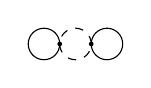
\begin{tikzpicture}
            \draw[dashed] (0,0) circle (0.2);
            \draw (0.4,0) circle (0.2);
            \draw (-0.4,0) circle (0.2);
            \fill (0.2,0) circle (0.03);
            \fill (-0.2,0) circle (0.03);
        \end{tikzpicture}}
        & + &
        \raisebox{-.4\height}{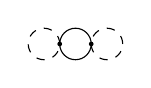
\begin{tikzpicture}
            \draw (0,0) circle (0.2);
            \draw[dashed] (0.4,0) circle (0.2);
            \draw[dashed] (-0.4,0) circle (0.2);
            \fill (0.2,0) circle (0.03);
            \fill (-0.2,0) circle (0.03);
        \end{tikzpicture}}
        & + &
        \raisebox{-.4\height}{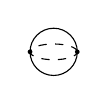
\begin{tikzpicture}
            \draw (0,0) circle (0.3);
            \draw[dashed] (0,0) ellipse (0.3 and 0.1);
            \fill (0.3,0) circle (0.03);
            \fill (-0.3,0) circle (0.03);
        \end{tikzpicture}}
        & + & \cdots\\
        \;= & \displaystyle\frac{1}{4}\frac{-\lambda}{m^2M^2} &+& \displaystyle\frac{1}{16}\frac{\lambda^2}{m^4M^4} &+& \displaystyle\frac{1}{16}\frac{\lambda^2}{m^4M^4} &+& \displaystyle\frac{1}{8}\frac{\lambda^2}{m^4M^4} &+& \cdots
    \end{matrix}
\end{align}
We can also compute expectation values, for example:
\begin{equation}
    \begin{array}{*{13}{>{\displaystyle}c}}
        \expval{\phi^2} &=&
        \raisebox{-.4\height}{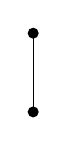
\begin{tikzpicture}
            \draw (0,0.5) -- (0,-0.5);
            \fill (0,0.5) circle (0.07);
            \fill (0,-0.5) circle (0.07);
        \end{tikzpicture}}
        &+&
        \raisebox{-.4\height}{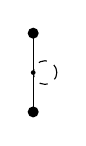
\begin{tikzpicture}
            \draw (0,0.5) -- (0,-0.5);
            \fill (0,0.5) circle (0.07);
            \fill (0,-0.5) circle (0.07);
            \draw[dashed] (0.15,0) circle (0.15);
            \fill (0,0) circle (0.03);
        \end{tikzpicture}}
        &+&
        \raisebox{-.4\height}{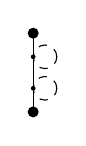
\begin{tikzpicture}
            \draw (0,0.5) -- (0,-0.5);
            \fill (0,0.5) circle (0.07);
            \fill (0,-0.5) circle (0.07);
            \draw[dashed] (0.15,0.2) circle (0.15);
            \fill (0,0.2) circle (0.03);
            \draw[dashed] (0.15,-0.2) circle (0.15);
            \fill (0,-0.2) circle (0.03);
        \end{tikzpicture}}
        &+&
        \raisebox{-.4\height}{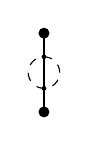
\begin{tikzpicture}
            \draw (0,0.5) -- (0,-0.5);
            \fill (0,0.5) circle (0.07);
            \fill (0,-0.5) circle (0.07);
            \draw[dashed] (0,0) circle (0.2);
            \fill (0,0.2) circle (0.03);
            \fill (0,-0.2) circle (0.03);
        \end{tikzpicture}}
        &+&
        \raisebox{-.4\height}{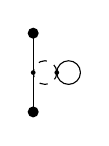
\begin{tikzpicture}
            \draw (0,0.5) -- (0,-0.5);
            \fill (0,0.5) circle (0.07);
            \fill (0,-0.5) circle (0.07);
            \draw (0.45,0) circle (0.15);
            \fill (0.3,0) circle (0.03);
            \draw[dashed] (0.15,0) circle (0.15);
            \fill (0,0) circle (0.03);
        \end{tikzpicture}}
        &+&\cdots \\\\
        &=& \frac{1}{m^2} &+& \frac{1}{2}\frac{-\lambda}{m^4M^2} &+& \frac{1}{4} \frac{\lambda^2}{m^6M^4} &+& \frac{1}{2}\frac{\lambda^2}{m^6M^4} &+& \frac{1}{4} \frac{\lambda^2}{m^6M^4} &+& \cdots
    \end{array}
\end{equation}
Note that we have no disconnected vacuum diagrams here because we divided by \(Z\) in \(\expval{\cdot}\).

Let's compute these results in a different way. We will briefly include \(\hbar\) in our calculations. We define the \emph{effective action} \(S_{\text{eff}}\) for \(\phi\) by the result of doing just the \(\chi\) path integral:
\begin{align}
    e^{-S_{\text{eff}}/\hbar} &= \int_\RR\dd{\chi} e^{-S(\phi,\chi)/\hbar}\\
    \intertext{We can actually calculate this integral exactly for our choice of \(S(\phi,\chi)\):}
    &= e^{-m^2\phi^2/2} \sqrt{\frac{2\pi\hbar}{M^2+\lambda\phi^2/2}}
\end{align}
So we have:
\begin{align}
    S_{\text{eff}} &= - \hbar\log\left[ e^{-m^2\phi^2/2} \sqrt{\frac{2\pi\hbar}{M^2+\lambda\phi^2/2}} \right] \\
    &= \frac{m^2\phi^2}{2} + \frac{\hbar}{2}\log\left( 1 + \frac{\lambda\phi^2}{2M^2} \right) + \underbrace{\frac{\hbar}{2}\log\left( \frac{M^2}{2\pi\hbar} \right)}_{\mathclap{\text{independent of \(\phi\) so drop it}}}\\
    &= \frac{m^2\phi^2}{2} + \frac{\hbar\lambda}{4M^2}\phi^2 - \frac{\hbar^2\lambda^2}{16M^4}\phi^4 + \frac{\hbar\lambda^3}{48M^6}\phi^6 + \dots\\
    &= \frac{m^2_{\text{eff}}\phi^2}{2} + \frac{\lambda_4\phi^4}{4!} + \frac{\lambda_6\phi^6}{6!} + \dots
\end{align}
where \(m^2_{\text{eff}} = m^2 + \frac{\hbar\lambda}{4M^2}\), \(\lambda_4 = - \frac{\hbar\lambda^24!}{16M^4}\), and so on.

Integrating out \(\chi\) has shifted the effective mass of \(\phi\). It has also produced an infinite series of new \(\phi\) interactions. These effects are quantum in the sense that they vanish as \(\hbar = 0\). More generically, we'd start with an action containing arbitrarily many vertices for \(\phi\) and \(\chi\):
\begin{equation}
    S(\phi,\chi) = \sum_{i,j=1}^\infty \frac{\lambda_{i,j}\phi^{2i}\chi^{2j}}{i!j!}
\end{equation}
Then integrating out \(\chi\) will shift the values of all of the \(\phi\) vertices, \(\lambda_{i,0} \rightarrow \lambda_{i,0}^{\text{eff}}\). These shifts will be proportional to polynomial powers of \(\hbar\). We will usually only be able to carry out the \(\chi\) integral perturbatively. Lets return to the simple action and do this.

If we just do a \(\chi\) integral, the Feynman rules are like before, except that we can have external \(\phi\)s, which have to be counted explicitly, but can't have any \(\phi\) propagators (unless they are between two external \(\phi\)s):
\begin{figure}[H]
    \centering
    \begin{tikzpicture}
        \draw[dashed] (0,0) node[left] {\(\chi\)} -- (2,0) node[right] {\(\chi\)};
        \node at (1,-0.5) {\(\frac{1}{M^2}\)};
        \draw (3.5,-0.2) -- (4.5,0.2) node[right] {\(\phi\)};
        \fill (4.5,0.2) circle (0.07);
        \node at (4,-0.5) {\(\phi\)};
        \draw (6,0) node[left] {\(\phi\)} -- (8,0) node[right] {\(\phi\)};
        \fill (6,0) circle (0.07);
        \fill (8,0) circle (0.07);
        \fill (7,0) circle (0.04);
        \node at (7,-0.5) {\(-m^2\)};
        \draw (10.5,0) arc (-90:-45:1.5) node[above] {\(\phi\)};
        \draw (10.5,0) arc (-90:-135:1.5) node[above] {\(\phi\)};
        \draw[dashed] (10.5,0) arc (90:135:1.5) node[below] {\(\chi\)};
        \draw[dashed] (10.5,0) arc (90:45:1.5) node[below] {\(\chi\)};
        \draw[fill] (10.5,0) circle (0.03) node[below] {\(\frac{-\lambda}{2}\)};
        \fill ({10.5-1.5/sqrt(2)},{1.5-1.5/sqrt(2)}) circle (0.07);
        \fill ({10.5+1.5/sqrt(2)},{1.5-1.5/sqrt(2)}) circle (0.07);
    \end{tikzpicture}
\end{figure}
With these rules we obtain:
\begin{equation}
    \begin{array}{*{11}{>{\displaystyle}c}}
        -S_{\text{eff}}(\phi) &=&
        \raisebox{-.4\height}{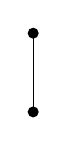
\begin{tikzpicture}
            \draw (0,0.5) -- (0,-0.5);
            \fill (0,0.5) circle (0.07);
            \fill (0,-0.5) circle (0.07);
        \end{tikzpicture}}
        &+&
        \raisebox{-.4\height}{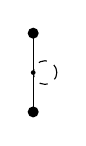
\begin{tikzpicture}
            \draw (0,0.5) -- (0,-0.5);
            \fill (0,0.5) circle (0.07);
            \fill (0,-0.5) circle (0.07);
            \draw[dashed] (0.15,0) circle (0.15);
            \fill (0,0) circle (0.03);
        \end{tikzpicture}}
        &+&
        \raisebox{-.4\height}{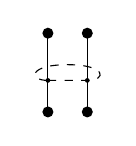
\begin{tikzpicture}
            \draw[dashed] (-0.25,-0.1) -- (0.25,-0.1)
                .. controls (0.5,-0.1) and (0.5,0.1) .. (0,0.1)
                .. controls (-0.5,0.1) and (-0.5,-0.1)
                .. cycle;
            \draw (-0.25,0.5) -- (-0.25,-0.5);
            \draw (0.25,0.5) -- (0.25,-0.5);
            \fill (0.25,0.5) circle (0.07);
            \fill (0.25,-0.5) circle (0.07);
            \fill (-0.25,0.5) circle (0.07);
            \fill (-0.25,-0.5) circle (0.07);
            \fill (0.25,-0.1) circle (0.03);
            \fill (-0.25,-0.1) circle (0.03);
        \end{tikzpicture}}
        &+&
        \raisebox{-.4\height}{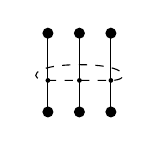
\begin{tikzpicture}
            \draw[dashed] (-0.4,-0.1) -- (0.4,-0.1)
                .. controls (0.65,-0.1) and (0.65,0.1) .. (0,0.1)
                .. controls (-0.65,0.1) and (-0.65,-0.1)
                .. cycle;
            \draw (-0.4,0.5) -- (-0.4,-0.5);
            \draw (0,0.5) -- (0,-0.5);
            \draw (0.4,0.5) -- (0.4,-0.5);
            \fill (0.4,0.5) circle (0.07);
            \fill (0.4,-0.5) circle (0.07);
            \fill (0,0.5) circle (0.07);
            \fill (0,-0.5) circle (0.07);
            \fill (-0.4,0.5) circle (0.07);
            \fill (-0.4,-0.5) circle (0.07);
            \fill (0.4,-0.1) circle (0.03);
            \fill (0,-0.1) circle (0.03);
            \fill (-0.4,-0.1) circle (0.03);
        \end{tikzpicture}}
        &+&\cdots\\\\
        &=& \frac{-m^2\phi^2}{2} &+& \frac{-\lambda}{4M^2}\phi^2 &+& \frac{\lambda^2}{16M^4}\phi^4 &+& \cdots
    \end{array}
\end{equation}
Note that only connected diagrams because \(S_{\text{eff}}(\phi)\) is the logarithm of the path integral. We see that the new vertices in \(S_{\text{eff}}(\phi)\) and the shift \(m^2\rightarrow m^2_{\text{eff}}\) have been generated by loops of the \(\chi\) field (in this case, just one loop).

We can use our \emph{effective field theory} to compute \(Z\) and all correlation functions where the operator insertions depend only on \(\phi\):
\begin{equation}
    \expval{\mathcal{O}_1(\phi)\dots\mathcal{O}_n(\phi)}_{S(\phi,\chi)} = \expval{\mathcal{O}_1(\phi)\dots\mathcal{O}_n(\phi)}_{S_{\text{eff}}(\phi)}
\end{equation}

It's better to use \(S_{\text{eff}}\) if we are interested in many different correlation functions. A general principle to adhere to is: ``We should describe physics using just those degrees of freedom that are relevant to the experiments that we are conducting.''

If correlation functions involve both \(\phi\) and \(\chi\), we require the full interacting theory.

\lecture{22/01/16}
\section{QFT in one dimension}
When \(d=1\), there are two topological possibilities for the space \(\mathcal{M}\) on which our QFT lives, if we require that \(\mathcal{M}\) is compact and connected:
\begin{itemize}
    \item \(\mathcal{M}=I=[0,T]\):
        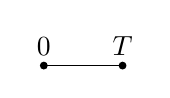
\begin{tikzpicture}
            \draw (0,0) node[above] {\(0\)} -- (1,0) node[above] {\(T\)};
            \fill (0,0) circle (0.05);
            \fill (1,0) circle (0.05);
        \end{tikzpicture}
    \item \(\mathcal{M}=S^1\):
        \raisebox{-.2\height}{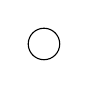
\begin{tikzpicture}
            \draw (0,0) circle (0.2);
        \end{tikzpicture}}
\end{itemize}
In both cases we will use \(t\) as a coordinate on \(\mathcal{M}\).

A standard choice of fields on \(\mathcal{M}\) is a map \(x:\mathcal{M}\to\mathcal{N}\), where \((\mathcal{N},g)\) is a Riemannian manifold.
\begin{figure}[H]
    \centering
    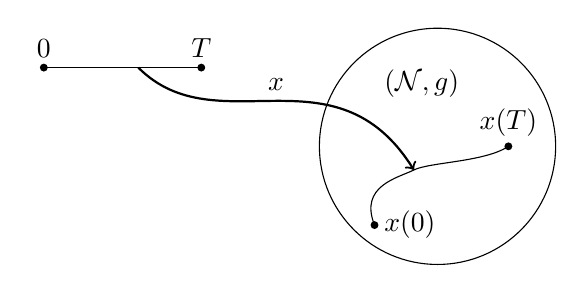
\begin{tikzpicture}
        \draw (0,0) node[above] {\(0\)} -- (2,0) node[above] {\(T\)};
        \fill (0,0) circle (0.05);
        \fill (2,0) circle (0.05);

        \draw (5,-1) circle (1.5);
        \node at (4.8,-0.2) {\((\mathcal{N},g)\)};
        \draw (4.2, -2) node[right] {\(x(0)\)} .. controls (4, -1.5) and (4.5,-1.4) .. (4.7,-1.3) 
        .. controls (4.9,-1.2) and (5.6,-1.2) .. (5.9,-1) node[above] {\(x(T)\)};
        \fill (4.2,-2) circle (0.05);
        \fill (5.9,-1) circle (0.05);

        \draw[thick,->] (1.2,0) .. controls (2.2,-1) and (3.7,0.3) .. (4.7,-1.3) node[midway, above] {\(x\)};
    \end{tikzpicture}
\end{figure}
If we let \(x^a\) for \(a = 1,\dots\dim(\mathcal{N}\) be local coordinates on \(\mathcal{N}\), and let \(V:\mathcal{N}\to\RR\) be a function on \(\mathcal{N}\), then a common choice of action for our QFT is:
\begin{equation}
    S[x] = \int_\mathcal{M}\left[ \frac{1}{2}g_{ab}\dot{x}^a\dot{x}^b + V(x) \right]\dd{t}
\end{equation}
where \(x^a = x^a(t)\) and \(\dot{x}^a = \dv{x^a}{t}\).

We might think that we should include a square root; see later for an explanation about this.

In quantum mechanics, we interpret \(\mathcal{N}\) as ``our universe'' and \(\mathcal{M}\) (or its image \(x(\mathcal{m})\subset\mathcal{N}\) as the worldline of a particle. In contrast, in this course we will view \(\mathcal{M}\) as ``our universe''. In this context, \(\mathcal{N}\) is called the \emph{target space}, and our model is a \emph{non-linear sigma model}.
\begin{eg}
    In pion physics, we have a field \(\pi:\mathcal{M}\to\mathcal{N} = SU(2)\times SU(2)/SU(2)\).
\end{eg}
\begin{eg}
    In string theory, we have \(x:\mathcal{M}\to CY\) (a Calabi-Yau manifold).
\end{eg}

If we vary \(S[x]\), we obtain the following Euler-Lagrange equation:
\begin{equation}
    \dv[2]{x^a}{t} + \Gamma^a_{bc}\dot{x}^b\dot{x}^c = - g^{ab}\partial_bV
\end{equation}
or, put another way, \(\vb{F} = -m\vb{a}\) (the minus sign is present because we are taking \(\mathcal{M}\) to have Euclidean time).

\subsection{Quantum mechanics}
Usually in QM, we pick a Hilbert space \(\mathcal{H}\) and a Hamiltonian \(H:\mathcal{H}\to\mathcal{H}\). In the present context, it is natural to pick \(\mathcal{H}=L^2(\mathcal{N})\) (the space of square-integrable functions on \(\mathcal{N}\)), and \(H = \frac{1}{2}\Delta + V\), where \(\Delta = \frac{1}{\sqrt{g}}\pdv{x^a}\left( g^{ab}\sqrt{g}\pdv{x^b} \right)\) is the Laplacian on \(\mathcal{N}\). The amplitude for a particle to travel from
\(y_0\in\mathcal{N}\) to \(y_1\in\mathcal{N}\) in a time \(T\) would be:
\begin{equation}
    \underbrace{\mel{y_1}{e^{-HT}}{y_0}}_{\text{Heisenberg picture}} 
    =
    \underbrace{\braket{y_1;T}{y_0;0}}_{\text{Schr\"odinger picture}}
\end{equation}
This is equivalent to \(K_T(y_1,y_0)\), where \(K_t(y_1,y_0)\) is the \emph{heat kernel}, defined to be the solution to:
\begin{equation}
    \pdv{t}K_t(y_1,y_0) = HK_t(y_1,y_0)
    ,\quad
    K_0(y_1,y_0) = \delta^n(y_1-y_0)
\end{equation}
Note again that this is in Euclidean signature. If we take \(t\to-it\) and include \(\hbar\) we obtain the familiar \(i\hbar\pdv{K_t}{t}=HK_t\).

In the case \((\mathcal{N},g) = (\RR^n,\delta)\) and \(V=0\), we have:
\begin{equation}
K_t(y_1,y_0) = \frac{1}{(2\pi t)^{n/2}}\exp\left( -\frac{|y_0-y_1|^2}{2t} \right)
\end{equation}
We can get a path integral interpretation by breaking the interval \([0,T]\) into many steps of length \(\Delta t = T/N\).
\begin{align}
    \mel{y_1}{e^{-HT}}{y_0}
    &= \mel{y_1}{e^{-H\Delta t}e^{-H\Delta t}\dots e^{-H\Delta t}}{y_0} \\
    &= \int \dd[n]{x_1}\dots\dd[n]{x_{N-1}} \mel{y_1}{e^{-H\Delta t}}{x_{N-1}} \bra{x_{N-1}} \dots \ket{x_1} \mel{x_1}{e^{-H\Delta t}}{x_{N-1}} \\
    &= \int \dd[n]{x_1}\dots\dd[n]{x_{N-1}} K_{\Delta t}(y_1,x_{N-1}) \dots K_{\Delta t}(x_1,y_0)
\end{align}
Therefore in flat space we have:
\begin{equation}
    K_T(y_1,y_0) = \int \prod_{i=1}^N \frac{\dd[n]{x_i}}{(2\pi\Delta t)^{n/2}}\exp\left[ -\frac{|x_{i+1}-x_i|^2}{2\Delta t} \right]
\end{equation}
Let's take off our mathematician hats (in a way that will thankfully be temporary in this course), and take the limit as \(\Delta t\to 0\) with \(N\Delta t\) fixed. We can write:
\begin{equation}
    \Dd{x} \stackrel{\disapprove}{=} \lim_{\substack{N\to\infty\\\Delta t\to0}} \prod_{i=1}^N \frac{\dd[n]{x_i}}{(2\pi\Delta t)^{n/2}}
\end{equation}
and:
\begin{equation}
    S[x] \stackrel{\disapprove}{=} \lim_{\substack{N\to\infty\\\Delta t\to0}} \sum_{i=1}^{N-1}\frac{1}{2}\left( \frac{|x_{i+1}-x_i|}{\Delta t} \right)^2\Delta_t \stackrel{\disapprove}{=}
    \int^T_0 \dd{t}\frac{1}{2}|\dot{x}|^2
\end{equation}
Then we recover the interpretation that:
\begin{equation}
    K_T(y_1,y_0) = \int_{\mathrlap{C_I[y_1,y_0]}} \;\; \Dd{x} e^{-S[x]}
\end{equation}
where \(C_I[y_1,y_0]\) is the space of all continuous maps \(x:I\to\mathcal{N}\) such that \(x(0) = y_0\) and \(x(T) = y_1\). So this is a sum over all possible paths from \(y_0\) to \(y_1\):
\begin{figure}[H]
    \centering
    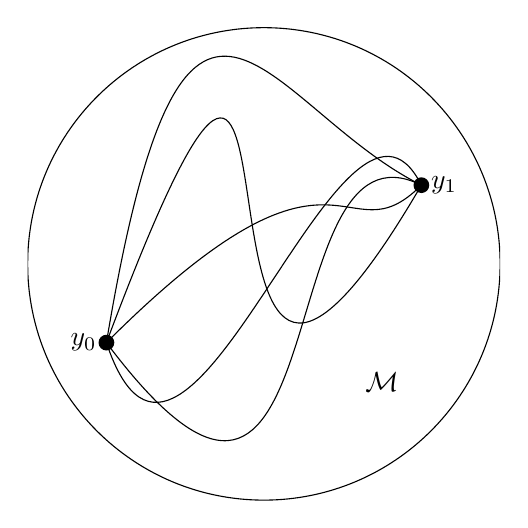
\begin{tikzpicture}
        \clip (-3,-3) rectangle (3,3);
        \draw (0,0) circle (3);
        \fill (-2,-1) circle (0.1) node[left] {\(y_0\)};
        \fill (2,1) circle (0.1) node[right] {\(y_1\)};
        \draw (-2,-1) .. controls (-1,-4) and (1,3) .. (2,1);
        \draw (-2,-1) .. controls (1,2) and (1,0) .. (2,1);
        \draw (-2,-1) .. controls (-1,5) and (0,2) .. (2,1);
        \draw (-2,-1) .. controls (1,-5) and (0,2) .. (2,1);
        \draw (-2,-1) .. controls (1,7) and (-1.5,-5) .. (2,1);
        \node at (1.5,-1.5) {\(\mathcal{M}\)};
    \end{tikzpicture}
\end{figure}

We define the partition function as the trace of the time evolution operator in the Hilbert space:
\begin{align}
    Z = \Tr_\mathcal{H} &= \int \dd[n]{y}\mel{y}{e^{-HT}}{y} \\
    &= \int\dd[n]{y}\int_{\mathrlap{C_I[y_1,y_0]}} \;\; \Dd{x} e^{-S[x]} \\
    &= \int\dd[n]{y}\int_{\mathrlap{C_{S^1}}} \;\; \Dd{x} e^{-S[x]}
\end{align}
So the partition function comes from a path integral for a QFT on a manifold \(\mathcal{M}\) (\(=S^1\)) without boundary.

A \emph{local operator} \(\mathcal{O}\) is one that depends on the values of the fields and their derivatives at just a single time \(t\in\mathcal{M}\). As a simple example, suppose \(\mathcal{O}\) depends on just \(x(t)\). Then we have:
\begin{align}
    \mel{y_1}{\hat{\mathcal{O}}(t)}{y_0} &= \mel{y_1}{e^{-H(T-t)}\hat{\mathcal{O}}e^{-Ht}}{y_0} \\
    &= \int \dd[n]{x_0} \mel{y_1}{e^{-H(T-t)}\hat{\mathcal{O}}}{x_0} \mel{x_0}{e^{-Ht}}{y_0} \\
    &= \int \dd[n]{x_0} K_{T-t}(y_1,x_0)K_t(x_0,y_0) \mathcal{O}(x_0) \\
    &= \int \dd[n]{x_0} \int_{\mathrlap{C_{I_2}[y_1,x_0]}} \;\; \Dd{x} e^{-S[x]} \mathcal{O}(x_0) \int_{\mathrlap{C_{I_1}[x_0,y_0]}} \;\; \Dd{x} e^{-S[x]} \\
    &= \int_{\mathrlap{C_I[y_1,y_0]}} \;\; \Dd{x} e^{-S[x]} \mathcal{O}(x(t))
\end{align}

\end{document}
